\documentclass[10pt]{article}
\usepackage[utf8]{inputenc}
\usepackage[spanish]{babel}
\usepackage[usenames,dvipsnames,svgnames,table]{xcolor}
\usepackage{multirow}
\usepackage{diagbox}
\usepackage{booktabs}
\usepackage{anysize} 
\usepackage{hyperref}
\usepackage{helvet}
\renewcommand\refname{Referencias}
\marginsize{2cm}{2cm}{2.0cm}{2cm}
\usepackage{enumitem}
\usepackage{setspace}
\usepackage{scrextend}
\usepackage{amssymb}
\usepackage{mathtools}
\addtokomafont{labelinglabel}{\sffamily}

%% Graphics
\usepackage{graphicx}
\usepackage{color}
\usepackage{gensymb}
\usepackage{multirow}
\usepackage{caption}
\usepackage{float}
\graphicspath{{img/}}
\setlength{\parindent}{0cm}


\hypersetup{
	colorlinks=true,
	linkcolor=blue,
	filecolor=magenta,
	urlcolor=cyan,
	citecolor=blue
}





\begin{document}
	
	\title{Fundamentos de Bases de Datos \\
		Practica 7\\ Normalización de la Base de Datos
	} 
	\author{}
	\date{16 de Abril del 2019}
	\maketitle
	

El objetivo en esta práctica es normalizar la base de datos de acuerdo al caso 
de uso que hemmos venido usando. Normalizar la base de datos evita almacenar 
información redundante,  para esta practica se usa la tercera formal normal (3NF).

\section{Esquema relacional no normalizado}

\begin{figure}[H]
	\centering
	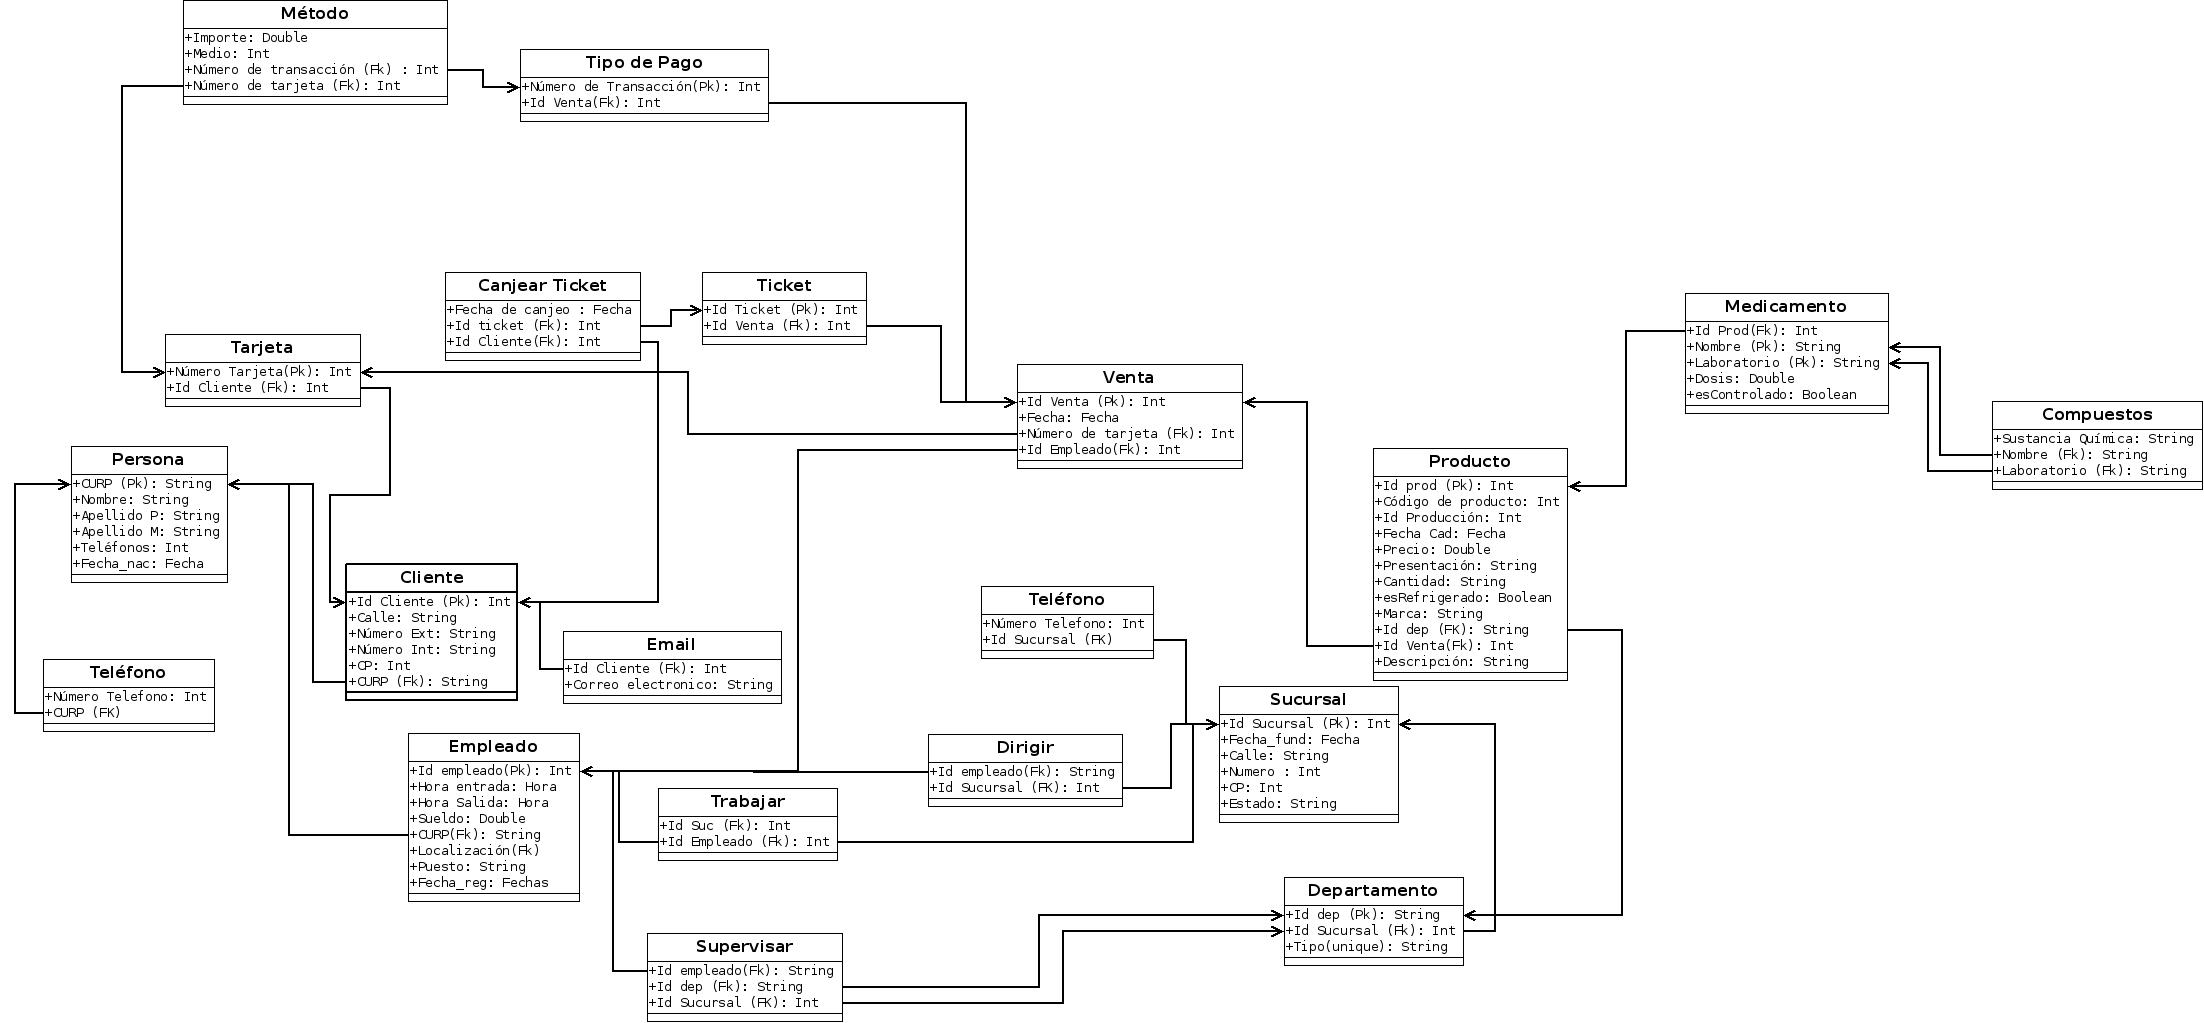
\includegraphics[scale=0.2 ]{practica05.jpeg}
	\caption{Esquema de la práctica anterior}
	\label{fg:esqA}
\end{figure}

\subsection{Cambios antes de la normalización}
\begin{itemize}
	\item Se trasforam la relación de Departamento a una relación de pertenencia
	entre una sucursal y un catálogo de tipos.
	\item Se corrigieron algunos errores de coincidencia de tipo, coincidencia
	de nombre.
\end{itemize}

\begin{figure}[H]
	\centering
	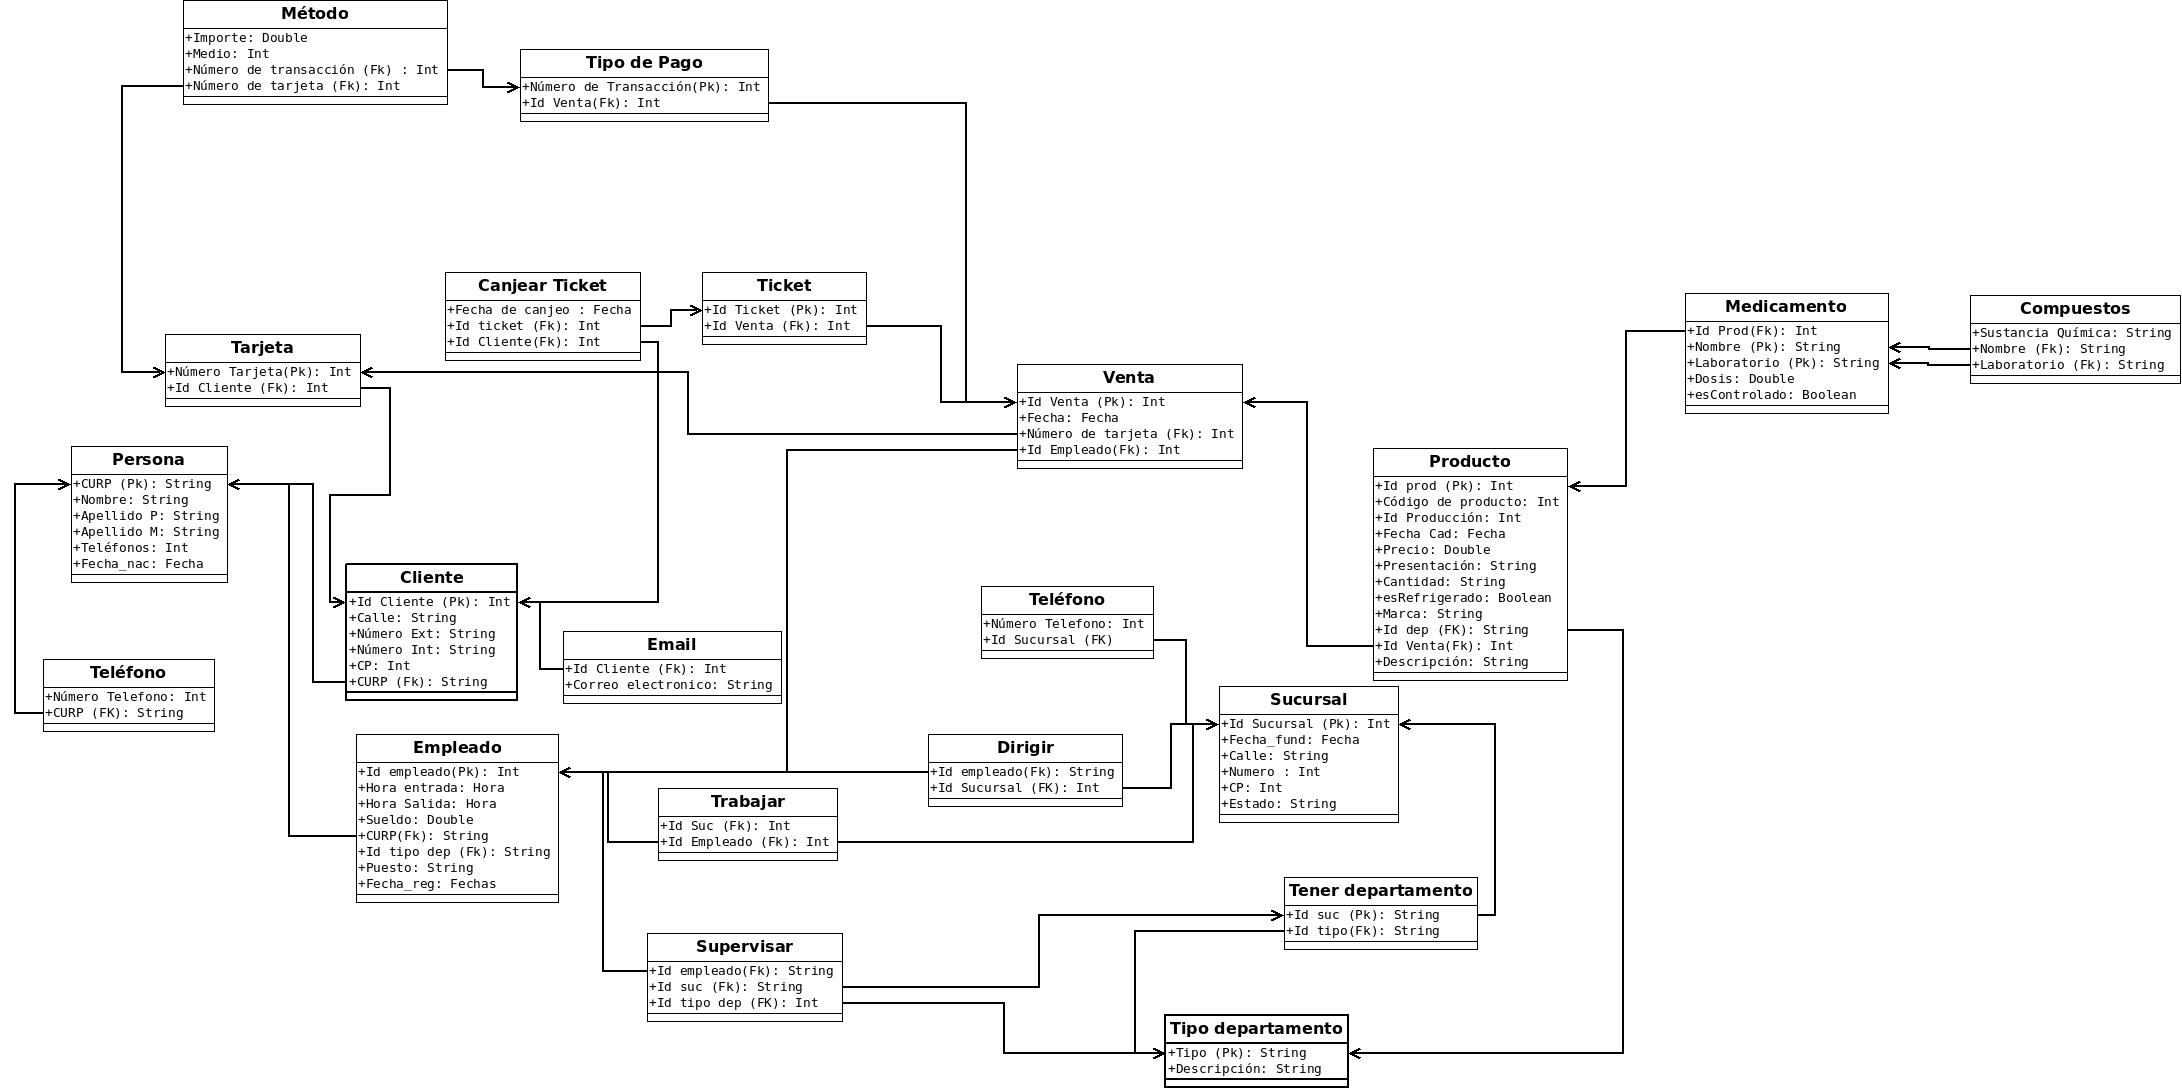
\includegraphics[scale=0.2 ]{practica07.jpeg}
	\caption{Esquema justo antes de la normalización}
	\label{fg:esNN}
\end{figure}

\section{Normalizando relaciones}

\subsection{Tablas claramente ya normalizadas}
Todas las relaciones con únicamente dos atributos ya está normalizadas, pues las
únicas dependencias funcionales que puede haber son las triviales o las inducidas
por llaves (un atributo determina al otro), y ninguna de estas es violación a la
tercara forma normal. En el equema, estas son
\begin{itemize}
	\item Tipo de pago
	\item Tarjeta
	\item Ticket
	\item Teléfono sucursal
	\item Teléfono persona
	\item Email
	\item Trabajar
	\item Dirigir
	\item Tener departamento
	\item Tipo departamento
\end{itemize}

\subsection{Tablas no tan claramente ya normalizadas}
\begin{enumerate}
	\item Método\\
	Tanto el importe como el medio sólo son valores para representar la cantidad
	de dinero, que no son únicos entre transacciones.\\
	Una transacción puede tener varios métodos de pago, así que tampoco
	puede determinar nada extra.\\
	Y una tarjeta puede tener varias instancias de método de pago, por lo que
	tampoco puede identificar a nada extra. \\
	Entonces las únicas dependencias funcionales que hay son triviales, por lo
	que la relación ya está normalizada.
	\item Canjear Ticket \\
	Pueden haber muchos canjeos el mismo día, así que la fecha no determina nada
	extra. \\ 
	Un cliente canjea varios tickets, así que tampoco el cliente determina
	nada extra. Y se pueden canjear varios tickets el mismo día, así que la 
	fecha con el cliente tampoco determina nada extra.\\
	El identificador del ticket es único, pues un ticket solo se canjea una vez.
	Entonces el identificador del ticket determina a todo lo demás, por lo que
	es llave.\\
	Entonces, si la relación es 
   \[\overbrace{{\textbf{CanjearTicket}}}^{\textbf{Ct}} 
   (
	   \overbrace{Fecha}^{F}, \overbrace{Id\_Ticket}^{T},
	   \overbrace{Id\_Cliente}^{C}
	)
	= 
	\textbf{Ct}(F, T, C)
	\]
	Las dependencias funcionales no triviales son 
	\[\mathcal{F} = \{T \rightarrow CF\}\]
	Que no violan la tercera forma normal (todas tiene una llave a la izquierda)
	.\\
	Por lo que la relación ya está normalizada.
	\item Venta \\
	Puede haber varias ventas por día, así que la fecha no determina nada extra.\\
	Una tarjeta puede usarse para varias ventas, así que el número de tarjeta no
	determna nada extra. Esas ventas pueden ser el mismo día, por lo que la fecha
	junto con el número de tarjeta no determina nada extra.\\
	Un empleado puede atender varias ventas así que el identificador de cliente
	no determina nada extra. También puede atender varias ventas el mismo día, y
	ventas diferentes que usaron la misma tarjeta así que el empleQdo junto con
	la fecha o la tarjeta no determinan nada extra.\\
	El identificador de venta es la llave, así que determina todo.\\
	Entonces, si la relación es 
	\[\overbrace{{\textbf{Venta}}}^{\textbf{V}} 
   (
	   \overbrace{Id\_Venta}^{I}, \overbrace{Fecha}^{F}, 
	   \overbrace{Num\_Tarjeta}^{T}, \overbrace{Id\_Empleado}^{E}
	)
	= 
	\textbf{V}(I, F, T, E)
	\]
	Las dependencias funcionales no triviales son 
	\[\mathcal{F} = \{I \rightarrow FTE\}\]
	Y como todas tienen una llave a la izquierda, no son violación de la tercera
	forma normal.\\
	Entonces la relación ya está normalizada.
	\item Medicamento \\
	El laboratorio puede tener varios medicamentos, así que no puede determinar
	nada extra. \\
	La dosis tampoco puede determinar nada extra, pues puede repetirse, al igual
	que la dosis con el laboratorio.\\
	Igualmente, la bandera sobre si es controlado no determina nada extra, así
	como tampoco esa bandera junto con el nombre del laboratorio o la dosis, o
	las tres juntas.\\
	El identificador del producto es único por lo que determinan todo y es llave
	, al igual que el nombre del medicamento.\\
	Entonces, si la relación es 
	\[\overbrace{{\textbf{Medicamento}}}^{\textbf{M}} 
   (
	   \overbrace{Id\_Prod}^{I}, \overbrace{Nombre}^{N}, 
	   \overbrace{Laboratorio}^{L}, \overbrace{Dosis}^{D},
	   \overbrace{Es\_Controlado}^{C}
	)
	= 
	\textbf{M}(I, N, L, D, C)
	\]
	Las dependencias funcionales no triviales son 
	\[\mathcal{F} = \{I \rightarrow NLDC, N \rightarrow ILDC\}\]
	Y como todas tienen una llave a la izquierda, no son violación de la tercera
	forma normal.\\
	Entonces la relación ya está normalizada.
	\item Compuestos \\
	El nombre y el laboratoio son parte de una llave foránea de medicamento. Un
	medicamento puede tener varios compuesto, así que no determina nada extra.\\
	La sustancia puede estar en varios medicamentos, así que tampoco es única,
	por lo que no puede determinar nada extra.\\
	Entonces sólo hay dependencias funcionales triviales y la relación ya está
	normalizada.
	\item Supervisar \\
	Un empleado puede supervisar varios departamentos, por lo que no determina nada
	extra.\\
	Un mismo tipo de departamento puede estar en varias sucursales, y un mismo
	empleado puede supervisar el mismo departamento en sucursales ddistintas,
	por lo que el departamento no determina nada, así como tampoco lo hacen el 
	departamento y el empleado.\\
	La sucursal puede tener varios departamentos, así que no puede determinar
	nada extra. Y en una misma sucursal un empleado puede supervisar varios
	departamentos, por lo que la sucursal y el empleado tampoco determinan nada
	extra.\\
	Cada departamento en una sucursal dada tiene sólo un supervisor, por lo que 
	el tipo de departamento con la sucursal determinan el empleado supervisor.
	Y como esta dependencia incluye a todos los atributos de la relación, es
	llave.\\
	Entonces, si la relación es 
	\[\overbrace{{\textbf{Supervisar}}}^{\textbf{S}} 
	(
		\overbrace{Id\_Empleado}^{E}, \overbrace{Id\_Departamento}^{D},
		\overbrace{Id\_Sucursal}^{Su}
	 )
	 = 
	 \textbf{S}(E, D, Su)
	 \]
	 Las dependencias funcionales no triviales son 
	 \[\mathcal{F} = \{DSu \rightarrow E\}\]
	 Y como la parte izquierda es una llave, no se viola la tercera forma normal.\\
	 Por lo que la relación ya está normalizada.
	\item Persona \\
	Tanto el Nombre como los dos Apellidos sólo son la representación atómica del
	atributo de Nombre Completo, que puede no ser único, así que no determina
	nada extra.\\
	De igual manera, varias personas nacen el mismo día, así que esta tampoco
	determina nada extra.\\
	Y sería demasiada coincidencia, pero es posible que personas con el mismo
	nombre nascan el mismo día, así que el nombre completo con la fecha de 
	nacimiento no determina nada extra.\\
	La CURP es la llave, por lo que determina todo lo demás.\\
	Entonces, si la relación es 
	\[\overbrace{{\textbf{Persona}}}^{\textbf{P}} 
   (
	   \overbrace{CURP}^{C}, \overbrace{Nombre}^{N}, 
	   \overbrace{Apellido P}^{Pa}, \overbrace{Apellido M}^{M},
	   \overbrace{Fecha\_Nac}^{F}
	)
	= 
	\textbf{P}(C, N, Pa, M, F)
	\]
	Las dependencias funcionales no triviales son 
	\[\mathcal{F} = \{C \rightarrow NPaMF\}\]
	Y como la parte izquierda es llave,  no hay violaciones a la tercera forma
	normal.\\
	Entonces la relación ya está normalizada.
	\item Cliente \\
	Tanto la calle, como los números y el CP son representación atómica del
	atributo de dirección. Y como puede haber varios clientes en una misma
	dirección, esta no determina nada extra.\\
	Tanto la CURP como el identificador de cliente son únicos, así que son
	llave.\\
	Entonces, si la relación es 
	\[\overbrace{{\textbf{Cliente}}}^{\textbf{C}} 
   (
	   \overbrace{Id\_Cliente}^{I}, \overbrace{Calle}^{Ca}, 
	   \overbrace{Numero Externo}^{Ne}, \overbrace{Numero Interno}^{Ni},
	   \overbrace{CP}^{Cp}, \overbrace{CURP}^{Cu}
	)
	= 
	\textbf{C}(I, Ca, Ne, Ni, Cp, Cu)
	\]
	Las dependencias funcionales no triviales son 
	\[\mathcal{F} = \{I \rightarrow CaNeNiCpCu, Cu \rightarrow ICaNeNiCp\}\]
	Y como la parte izquierda de ambas es llave, no hay violaciones a la tercera
	forma normal.\\
	Entonces la relación ya está normalizada.
\end{enumerate}

\subsection{Relacion Producto}

%\noindent \textbf{PRODUCTO}\textit{(Id\_Producto, Código\_Barras, Id\_Producción, %Fecha\_Cad, Precio, Presentación, Cantidad, esRefrigerado, Marca, Id\_Departamento, %Id\_Venta, Descripción)}\\



Para facilitar la definición de las dependencias funcionales de la relación Producto nos conviene etiquetarla de la siguiente manera:

\begin{align*}
\overbrace{ \textbf{PRODUCTO}}^{\textbf{{P}}}&(\overbrace{ Id\_Producto}^{\textbf{\textcolor{RoyalBlue}{A}}},\,\overbrace{Codigo\_Barras}^{\textbf{\textcolor{RoyalBlue}{B}}},\,\overbrace{Id\_Produccion}^{\textbf{\textcolor{RoyalBlue}{C}}},\,\overbrace{Fecha\_Cad}^{\textbf{\textcolor{RoyalBlue}{D}}},\,\overbrace{Precio}^{\textbf{\textcolor{RoyalBlue}{E}}},\,\overbrace{Presentacion}^{\textbf{\textcolor{RoyalBlue}{F}}},\\&\overbrace{Cantidad}^{\textbf{\textcolor{RoyalBlue}{G}}},\,\overbrace{esRefrigerado}^{\textbf{\textcolor{RoyalBlue}{H}}},\,\overbrace{Marca}^{\textbf{\textcolor{RoyalBlue}{I}}},\,\overbrace{Id\_Departamento}^{\textbf{\textcolor{RoyalBlue}{J}}},\,\overbrace{Id\_Venta}^{\textbf{\textcolor{RoyalBlue}{K}}},\,\overbrace{Descripcion}^{\textbf{\textcolor{RoyalBlue}{L}}})\\
&= \textbf{P}(\mathrm{A,B,C,D,E,F,G,H,I,J,K,L})
\end{align*}

%\overbrace{,}^{\textbf{\textcolor{Blue}{}}}
Las siguientes dependencias funcionales para esta relacion son:\\

$$\mathcal{F}=\mathrm{\{ BIFG \rightarrow E, BC \rightarrow D, B \rightarrow FGHI \}}$$

Para normalizar primero tenemos que calcular la cerradura para cada dependencia funcional en $\mathcal{F}$,\\


$\mathrm{\{\textcolor{RoyalBlue}{BIFG}\}+= \{\textcolor{RoyalBlue}{BIFG}EH\}}$\\

$\mathrm{\{\textcolor{RoyalBlue}{BC}\}+= \{\textcolor{RoyalBlue}{BC}FGHIDE\}}$\\

$\mathrm{\{\textcolor{RoyalBlue}{B}\}+= \{\textcolor{RoyalBlue}{B}FGHIE\}}$\\


Observamos que a la cerradura de BC es que contiene el mayor numero de atributos y unicamente le faltan algunos atributos, por lo tanto una llave para \textbf{P} es \underline{ABCJKL} \\

Lo siguiente es buscar violaciones a la tercera forma normal, para eso hay que ver que no aparezca la llave en las dependecias funcionales, observamos que las tres dependencias son violaciones a la 3NF, así que se toma una dependencia funcional con mas de un atributo a la izquierda para ver si alguno de los atributos es superfluo.\\

\subsubsection{Superfluos a la Izquierda}
\noindent Tomamos $\mathrm{BIFG \rightarrow E}$, luego verificamos si algun atributo a la izquierda es superfluo. \\
\begin{itemize}


\item ¿B es superfluo? $\mathrm{IFG \rightarrow E}$\\

$\mathrm{\{\textcolor{RoyalBlue}{IFG}\}+= \{\textcolor{RoyalBlue}{IFG}\}}$\\
 	
Como E no aparece en la cerradura de IFG, por lo tanto se concluye que B no es superfluo.\\

\item ¿I es superfluo? $\mathrm{BFG \rightarrow E}$\\

$\mathrm{\{\textcolor{RoyalBlue}{BFG}\}+= \{\textcolor{RoyalBlue}{BFG}HIE\}}$\\

E aparece en la cerradura de BFG, por lo tanto se concluye que I es superfluo.\\

\item ¿F es superfluo? $\mathrm{BIG \rightarrow E}$\\

$\mathrm{\{\textcolor{RoyalBlue}{BIG}\}+= \{\textcolor{RoyalBlue}{BIG}FHE\}}$\\

E aparece en la cerradura de BIG, por lo tanto se concluye que F es superfluo.\\

\item ¿G es superfluo? $\mathrm{BIF \rightarrow E}$\\

$\mathrm{\{\textcolor{RoyalBlue}{BIF}\}+= \{\textcolor{RoyalBlue}{BIF}GHE\}}$\\

E aparece en la cerradura de BIF, por lo tanto se concluye que G es superfluo.\\

\end{itemize}

\noindent Como resultado de buscar superfluos por la izquierda obtenemos una $\mathcal{F}$ nueva,\\

$$\mathcal{F}=\mathrm{\{ B \rightarrow E, BC \rightarrow D, B \rightarrow FGHI \}}$$ \\ 
y por la regla de la union obtenemos $$\mathcal{F}=\mathrm{\{ BC \rightarrow D, B \rightarrow FGHIE \}}$$ \\

\subsubsection{Superfluos por la derecha}

Tenemos a $\mathrm{B \rightarrow FGHIE}$ y buscamos elementos superfluos a la derecha.\\

\begin{itemize}
	\item ¿F es superfluo? $\mathrm{B \rightarrow GHIE}$ \\
	$$\mathcal{F}'=\mathrm{\{ BC \rightarrow D, B \rightarrow GHIE \}}$$\\
	Calculamos la cerradura de B usando a $\mathcal{F}'$\\
	$\mathrm{\{\textcolor{RoyalBlue}{B}\}+= \{\textcolor{RoyalBlue}{B}GHIE\}}$\\
	
	F no aparece en la cerradura de B, por lo tanto F no es superfluo.
	
	\item ¿G es superfluo? $\mathrm{B \rightarrow FHIE}$ \\
	$$\mathcal{F}'=\mathrm{\{ BC \rightarrow D, B \rightarrow FHIE \}}$$\\
	Calculamos la cerradura de B usando a $\mathcal{F}'$\\
	$\mathrm{\{\textcolor{RoyalBlue}{B}\}+= \{\textcolor{RoyalBlue}{B}FHIE\}}$\\
	
	G no aparece en la cerradura de B, por lo tanto G no es superfluo.
	
	\item ¿H es superfluo? $\mathrm{B \rightarrow FGIE}$ \\
	$$\mathcal{F}'=\mathrm{\{ BC \rightarrow D, B \rightarrow FGIE \}}$$\\
	Calculamos la cerradura de B usando a $\mathcal{F}'$\\
	$\mathrm{\{\textcolor{RoyalBlue}{B}\}+= \{\textcolor{RoyalBlue}{B}FGIE\}}$\\
	
	H no aparece en la cerradura de B, por lo tanto H no es superfluo.
	
	\item ¿I es superfluo? $\mathrm{B \rightarrow FGHE}$ \\
	$$\mathcal{F}'=\mathrm{\{ BC \rightarrow D, B \rightarrow FGHE \}}$$\\
	Calculamos la cerradura de B usando a $\mathcal{F}'$\\
	$\mathrm{\{\textcolor{RoyalBlue}{B}\}+= \{\textcolor{RoyalBlue}{B}FGHE\}}$\\
	
	I no aparece en la cerradura de B, por lo tanto I no es superfluo.
	
	\item ¿E es superfluo? $\mathrm{B \rightarrow FGHI}$ \\
	$$\mathcal{F}'=\mathrm{\{ BC \rightarrow D, B \rightarrow FGHI \}}$$\\
	Calculamos la cerradura de B usando a $\mathcal{F}'$\\
	$\mathrm{\{\textcolor{RoyalBlue}{B}\}+= \{\textcolor{RoyalBlue}{B}FGHI\}}$\\
	
	E no aparece en la cerradura de B, por lo tanto E no es superfluo.\\
	
\end{itemize}	
	Así que la $\mathcal{F}_{min}$ es,\\
	
	$$\mathcal{F}'_{min}= \mathrm{\{ BC \rightarrow D, B \rightarrow FGHIE \}}$$
	
	Esto quiere decir que las relaciones quedan como: \\
	
	$\mathrm{R_1(B,C,D)}\,\,\, con \,\,\, \mathrm{ BC \rightarrow D}$\\
	$\mathrm{R_2(B,F, G, H, I, E)}\,\,\, con \,\,\, \mathrm{ B \rightarrow FGHIE}$\\
	
	El siguiente paso es verificar si la llave esta en alguna relaciones obtenidas, como la llave no aparece en ninguna relación la solución es agregar otra relación que la contenga.\\
	
	
	$\mathrm{R_3(A,B,C,J,K,L)}\,\,\, con \,\,\, \mathrm{ ABCJKL \rightarrow ABCJKL}$\\


   $\therefore \,\, \mathrm{R_1, R_2, R_3} $  es la normalización en 3NF para la relación Producto. 
   
   
   \subsection{Relacion Empleado}
   Para la relación empleado se tiene:\\
   
   \begin{align*}
   \overbrace{ \textbf{EMPLEADO}}^{\textbf{{E}}}&(\overbrace{ Id\_empleado}^{\textbf{\textcolor{RoyalBlue}{ie}}},\,\overbrace{Hora\, entrada}^{\textbf{\textcolor{RoyalBlue}{he}}},\,\overbrace{Hora\, salida}^{\textbf{\textcolor{RoyalBlue}{hs}}},\,\overbrace{Sueldo}^{\textbf{\textcolor{RoyalBlue}{S}}},\,\overbrace{CURP}^{\textbf{\textcolor{RoyalBlue}{C}}},\,\overbrace{Id\_tipo\, dep}^{\textbf{\textcolor{RoyalBlue}{td}}},\overbrace{Puesto}^{\textbf{\textcolor{RoyalBlue}{P}}},\,\overbrace{Fecha\_reg}^{\textbf{\textcolor{RoyalBlue}{fr}}})\\
   &= \textbf{E}(ie,he,hs,S,C,td,P,fr)
   \end{align*}
   
   Se definen las siguientes dependecias funcionales para la relación Empleado\\
   
   $$\mathcal{F}=\{ tdfrP \rightarrow S,\, tdP \rightarrow hehs\}$$\\
   
   Calculamos la cerradura para cada una de las dependencias en $\mathcal{F}$\\
   
   $\{\textcolor{RoyalBlue}{tdfrP}\}+= \{\textcolor{RoyalBlue}{tdfrP}Shehs\}$\\
   
   $\{\textcolor{RoyalBlue}{tdP}\}+= \{\textcolor{RoyalBlue}{tdP}hehs\}$\\
   
   Una llave para \textbf{E} es \underline{ieCtdfrP}.\\
   
   Buscamos violaciones a la tercera forma normal, y encontramos que las dos son violaciones.\\
   
   \subsubsection{Superfluos a la Izquierda}
   
   Para buscar elementos superfluos a la izquierda elegimos la siguiente dependencia : $tdfrP \rightarrow S$\\
   
   \begin{itemize}
   	\item ¿td es superfluo? $frP \rightarrow S$\\
   	$\textcolor{RoyalBlue}{\{frP\}}+= \textcolor{RoyalBlue}{\{frP\}} $
   	
   	
   	S no aparece en la cerradura de $frP$, por lo tanto $td$ \underline{NO} es superfluo.\\
   	
   	\item ¿fr es superfluo? $tdP \rightarrow S$\\
   	$\{\textcolor{RoyalBlue}{tdP}\}+= \{\textcolor{RoyalBlue}{tdP}hehs\}$\\
   	
   	S no aparece en la cerradura de $tdP$, por lo tanto $fr$ \underline{NO} es superfluo.\\
   	
   	\item ¿P es superfluo? $tdfr \rightarrow S$\\
   	$\textcolor{RoyalBlue}{\{tdfr\}}+= \textcolor{RoyalBlue}{\{tdfr\}} $
   	
   	S no aparece en la cerradura de $tdfr$, por lo tanto $P$ \underline{NO} es superfluo.\\
   	
   	
   	$$\mathcal{F}_{min}=\{ tdfrP \rightarrow S,\, tdP \rightarrow hehs\}$$\\
   	
   	\subsubsection{Superfluos a la Derecha}
   	
   	Para buscar atributos superfluos por la derecha elegimos la siguiente dependencia que tine mas de un atributo a la derecha : $tdP \rightarrow hehs$
   	
   	
   	\begin{itemize}
   		\item ¿$he$ es superfluo? $tdP \rightarrow hs$\\
   		Se obtiene una $\mathcal{F'} = \{tdfrP \rightarrow S \,tdP \rightarrow hs\}$ y de aquí calculamos la cerradura para $tdP$\\
   		$\textcolor{RoyalBlue}{\{tdP\}}+= \{\textcolor{RoyalBlue}{tdP}hs\}$
   		$he$ no aparece en la cerradura de $tdP$, por lo tanto $he$ \underline{NO} es superfluo.\\
   		
   		\item ¿$hs$ es superfluo? $tdP \rightarrow he$\\
   		De aquí definimos una $\mathcal{F'} = \{tdfrP \rightarrow S \,tdP \rightarrow he\}$ y calculamos la cerradura para $tdP$\\
   		$\textcolor{RoyalBlue}{\{tdP\}}+= \{\textcolor{RoyalBlue}{tdP}he\}$
   		$hs$ no aparece en la cerradura de $tdP$, por lo tanto $hs$ \underline{NO} es superfluo.\\
   		
   		
   		
   		 
   		
   		
   	\end{itemize}
   
   Por lo tanto se concluye que la $\mathcal{F}_{min}$ es:
   
   \[\mathcal{F}_{min}=\{ tdfrP \rightarrow S,\, tdP \rightarrow hehs\}\]\\
   
   así que las relaciones serían\\
   
   $R_1(td,fr,P,S)$ con $ tdfrP \rightarrow S$  \\
   $R_2(td,P,he,hs)$ con $ tdP \rightarrow hehs $\\
   
   Pero de estas dos relaciones ninguna de ellas contiene a la llave, entonces agregamos una 
   nueva relación que la contenga $R_3(ie,C,td,fr,P)$ con  $ieCtdfrP \rightarrow ieCtdfrP$.\\
   	
   	$\therefore \,\, {R_1, R_2, R_3} $  es la normalización en 3NF para la relación Empleado.
   	
   \end{itemize}

    \subsection{Relacion Sucursal}
    La relación es 
    \[\overbrace{{\textbf{Sucursal}}}^{\textbf{S}} 
    (
	   \overbrace{Id\_Suc}^{I}, \overbrace{Fecha\_Fund}^{F},
	   \overbrace{Calle}^{C}, \overbrace{Numero}^{N}, Cp,
	   \overbrace{Estado}^{E}
	)
	= 
	\textbf{S}(I, F, C, N, Cp, E)
	\]
    Con las siguientes dependencias funcionales
    \[\mathcal{F} = \{I \rightarrow FCNCpE, Cp \rightarrow E\}\]
    Si bien existen dependencias funcionales que violan la tercera forma normal,
    sólo es una dependencia funcional que sólo concierne a dos atrbutos, por lo
    que so consideró que no vale la pena normalizar esta relación, puesto que el
    trabajo neesario para hacerlo es demasiado en comparación a la disminución de
	redundancia obtenida.
	
	\subsection{Esquema normalizado}
	\begin{figure}[H]
		\centering
		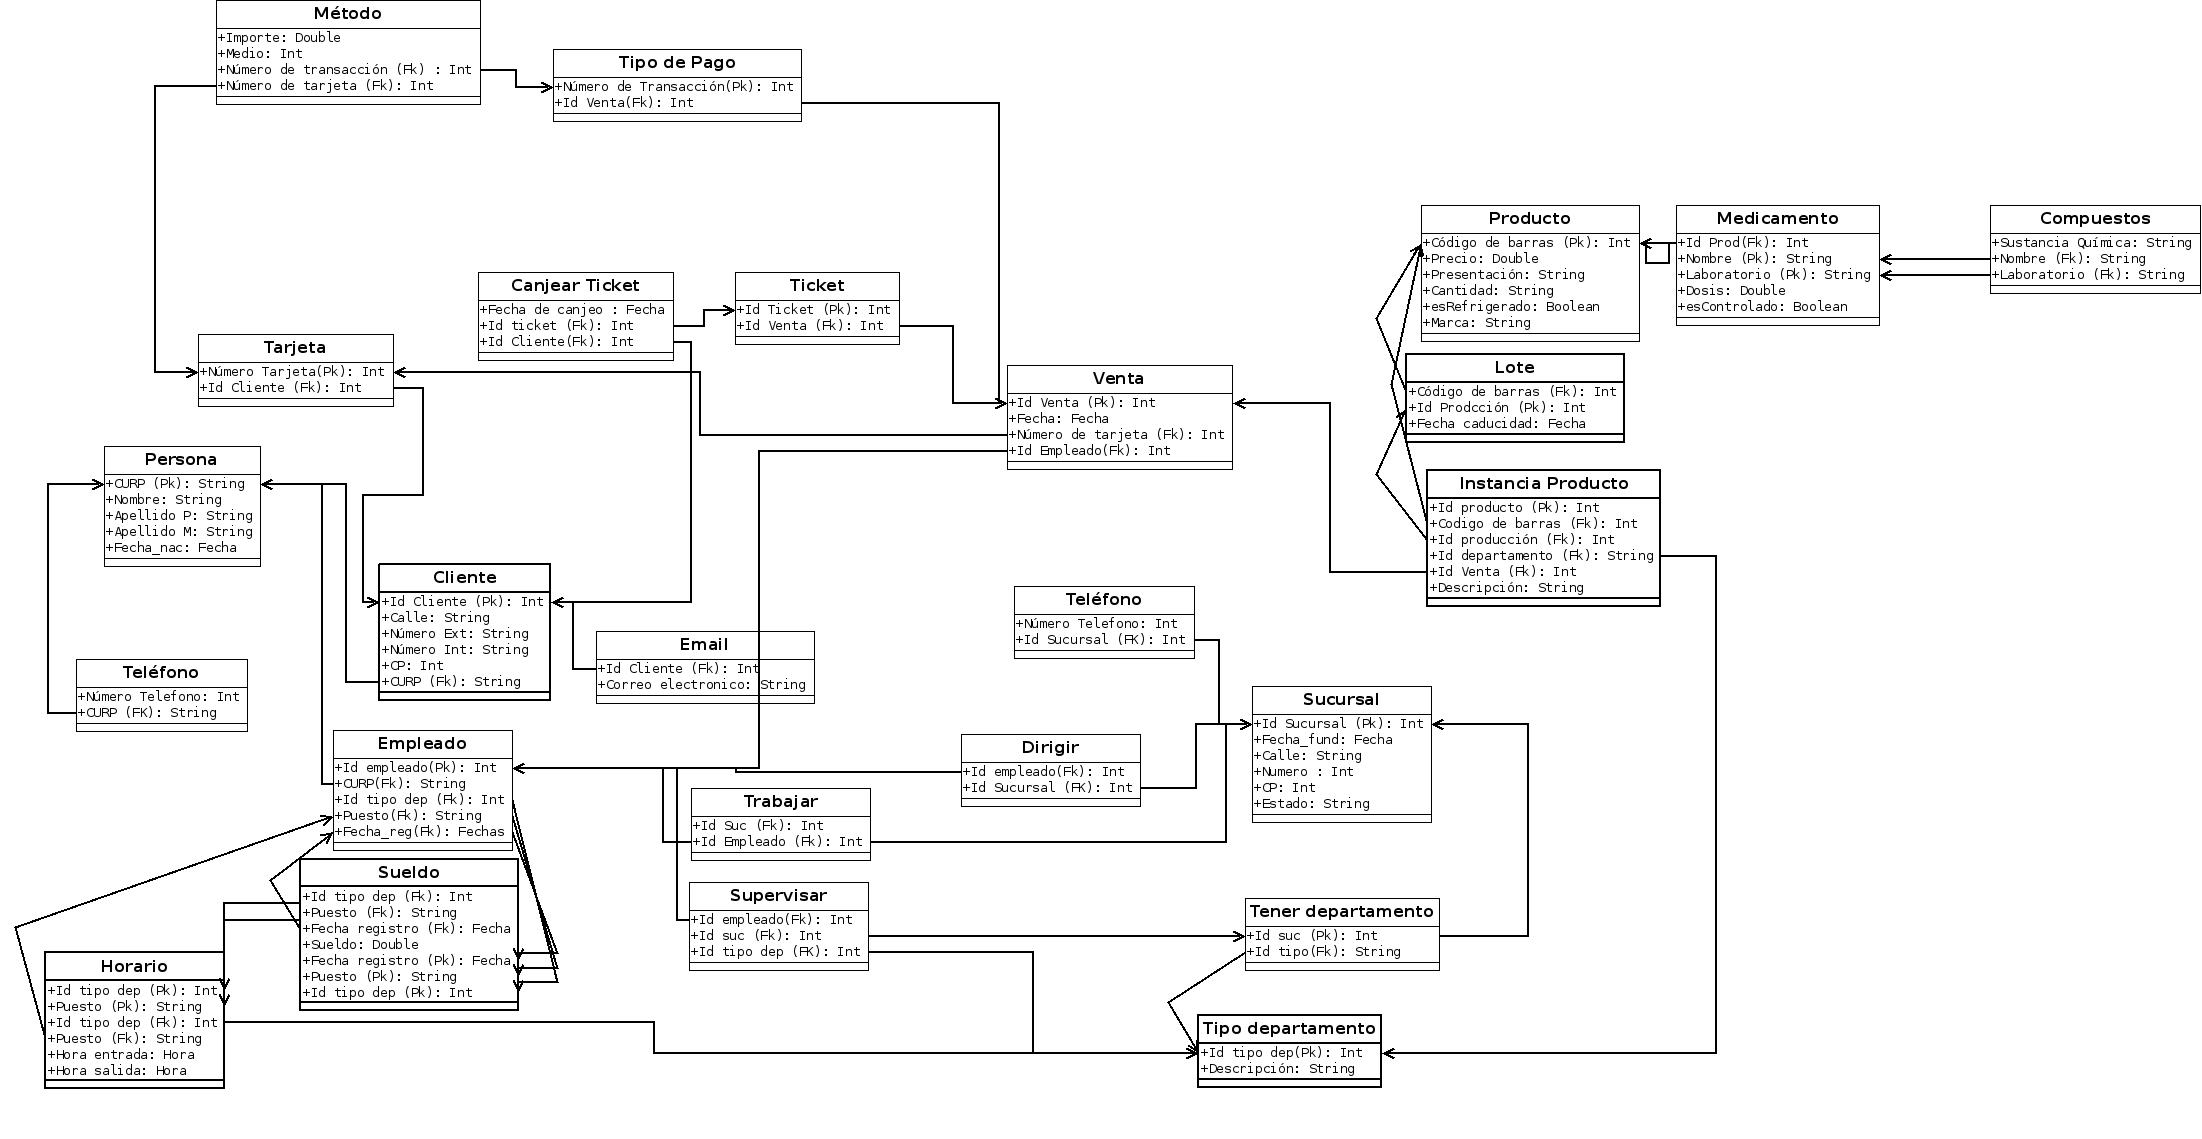
\includegraphics[scale=0.2]{practica07Norm.jpeg}
		\caption{Esquema normalizado}
		\label{fg:en}
	\end{figure}
	
	\section*{Preguntas extra}
	
	\subsection{Oracle Database Types}
	Para  responder a esto, consultamos en la página de Oracle la documentación
	de las verisones usadas, especificamente bajo las guías de \textit{Administración}
	en el apartado de \textit{\textbf{Database Concepts}}:
	    \begin{itemize}
	        \item \href{https://docs.oracle.com/en/database/oracle/oracle-database/18/
	        cncpt/database-concepts.pdf}{Oracle DB Enterprise Edition 18c}.
	        \item \href{https://docs.oracle.com/cd/B28359_01/server.111/b28318/datatype
	        .htm#CNCPT413}{Oracle DB Enterprise Edition 11g, Release 1}.
	    \end{itemize}

	\subsubsection{En la versión 18c}
	Se listan las siguientes categorías de tipos de datos:
	\begin{itemize}
	\small
	    \item Character Data Types [CHAR, VARCHAR2, NCHAR, NVARCHAR2]
        \item Numeric Data Types [NUMBER, BINARY\_FLOAT, BINARY\_DOUBLE]
        \item Datetime Data Types [DATE, TIMESTAMP, DATETIME(2)]
        \item Rowid Data Types [ROWID(categorizados como físicos, lógicos, foráneos ó 
              universales)]
        \item Format Models and Data Types //'moldes' de los tipos de datos como cadenas,
              metadatos
    \end{itemize}
	
	Aparte de estos, también menciona la existencia de \textit{raw}, \textit{large objects
	(LOBs)}, y \textit{collections}, junto con los tipos que se pueden acceder a través de 
	PL/SQL. \footnote{variables, 'constantes' ( Booleanos?), referencias y tipos, tanto 
	compuestos como definidos por el usuario.}
	
	\subsubsection{En la versión 11g}
	Se pueden encontrar las siguientes categorías y tipos de datos:
	\begin{itemize}
	\small
	    \item Character Data Types [CHAR, VARCHAR2, NCHAR, NVARCHAR2, LONG]
        \item Numeric Data Types [NUMBER, BINARY\_FLOAT, BINARY\_DOUBLE]
        \item Datetime Data Types [DATE, TIMESTAMP, DATETIME(2)]
        \item LOBs [BLOB, CLOB, NCLOB, BFILE]
        \item RAWs [RAW, LONG\_RAW]
        \item Rowid Data Types [ROWID, UROWID]
    \end{itemize}
	
	Vale la pena notar que LOB y RAW también existen el a versión 18c, aunque sólo se
	mencione su existencia. En esta documentación también aparecen como categorías los 
	\textit{ANSI, DB2, SQL/DS, XML, URI, Object y Object Views} pero recuperando la idea 
	de la documentación de la versión 18c, decidimos no listarlos como a los anteriores.
	
	\subsection{Restricciones para 'new\_name' (RENAME)}
	
	Consultamos  de nuevo en la página de Oracle la documentación de cada versión las 
	guías de\textit{Administración} pero esta vez en el apartado \textit{\textbf{SQL 
	Language Reference}}. En el caso de la versión 18c podríamos haber consultado el
	equivalente en PL/SQL pero en este no mencionaba nada sobre 'new\_name' concreto.
	    \begin{itemize}
	        \item \href{https://docs.oracle.com/en/database/oracle/oracle-database/18/
	        sqlrf/sql-language-reference.pdf}{Oracle DB Enterprise Edition 18c}.
	        \item \href{https://docs.oracle.com/cd/B28359_01/server.111/b28286/stateme
	        nts_9019.htm#SQLRF01608}{Oracle DB Enterprise Edition 11g, Release 1}.
	    \end{itemize}
    Nótese que en ambas aparece el mismo texto, con cási el mismo formato (es esto un
    copy-paste?):\\
    \textbf{new\_name}
    {Specify the new name to be given to the existing object. The new name must not
    already be used by another schema object in the same namespace and must follow
    the rules for naming schema objects.

    \textbf{Restrictions on Renaming Objects}
    Renaming objects is subject to the following restrictions:
    \begin{itemize}
        \item {You cannot rename a public synonym. Instead, drop the public synonym and
        then re-create the public synonym with the new name.}
        \item {You cannot rename a type synonym that has any dependent tables or 
        dependent valid user-defined object types.}
    \end{itemize}}
    
    Con lo cual debería quedar resuelta la pregunta.
	
\end{document}
